\chapter{Long Quotations}
Let's start with a long meaningless quotation so we can see how quotations are done.

\begin{quotation}
	Four score and seven years ago our fathers brought forth on this continent, a new nation, conceived in Liberty, and dedicated to the proposition that all men are created equal.
	
	Now we are engaged in a great civil war, testing whether that nation, or any nation so conceived and so dedicated, can long endure. We are met on a great battle-field of that war. We have come to dedicate a portion of that field, as a final resting place for those who here gave their lives that that nation might live. It is altogether fitting and proper that we should do this.
	
	But, in a larger sense, we can not dedicate -- we can not consecrate -- we can not hallow -- this ground. The brave men, living and dead, who struggled here, have consecrated it, far above our poor power to add or detract. The world will little note, nor long remember what we say here, but it can never forget what they did here. It is for us the living, rather, to be dedicated here to the unfinished work which they who fought here have thus far so nobly advanced. It is rather for us to be here dedicated to the great task remaining before us -- that from these honored dead we take increased devotion to that cause for which they gave the last full measure of devotion -- that we here highly resolve that these dead shall not have died in vain -- that this nation, under God, shall have a new birth of freedom -- and that government of the people, by the people, for the people, shall not perish from the earth.
\end{quotation} 
Now some text outside the quotation.
\section{Chemical Equations in \LaTeX}
If you need chemistry symbols you can use
\verb|\usepackage{mhchem}| which must be in the preamble of your main document.
They are made in the following way \verb|\ce{ H2O }| becomes \ce{ H2O }.
There is very little \ce{ O2 } in space.  
\section[Long Section Names]{Some section names are way to long to appear in the table of contents so you need to include a short title for the TOC}
This is an example of a section name that is too long.  You should shorten it if you can, but if you can't this long name will mess up the Table of Contents.  So there is an option to include a short title.  Put the short section nave version in square brackets before the actual (long) section name (in curly brackets).
Here is a random numbered list.
\begin{enumerate}
	\item one item that is long so we can see the hanging indent happen and because a hanging indent looks better, don't you think so?
	\item a second item, $2 \pi$
	
\end{enumerate}

\section{Double figures}
Sometimes it is useful to have two figures side by side. One way to do this is with a minipage environment. Here is an example of doing just that. Notice that I had to adjust the caption sizes to make the figures line up nicely. I used a \verb|\vspace| command to adjust the vertical spacing of the second figure. There are probably more elegant ways of doing this.

\begin{figure}[htb!]
	\centering
	\begin{minipage}{.45\textwidth}
		\centering
		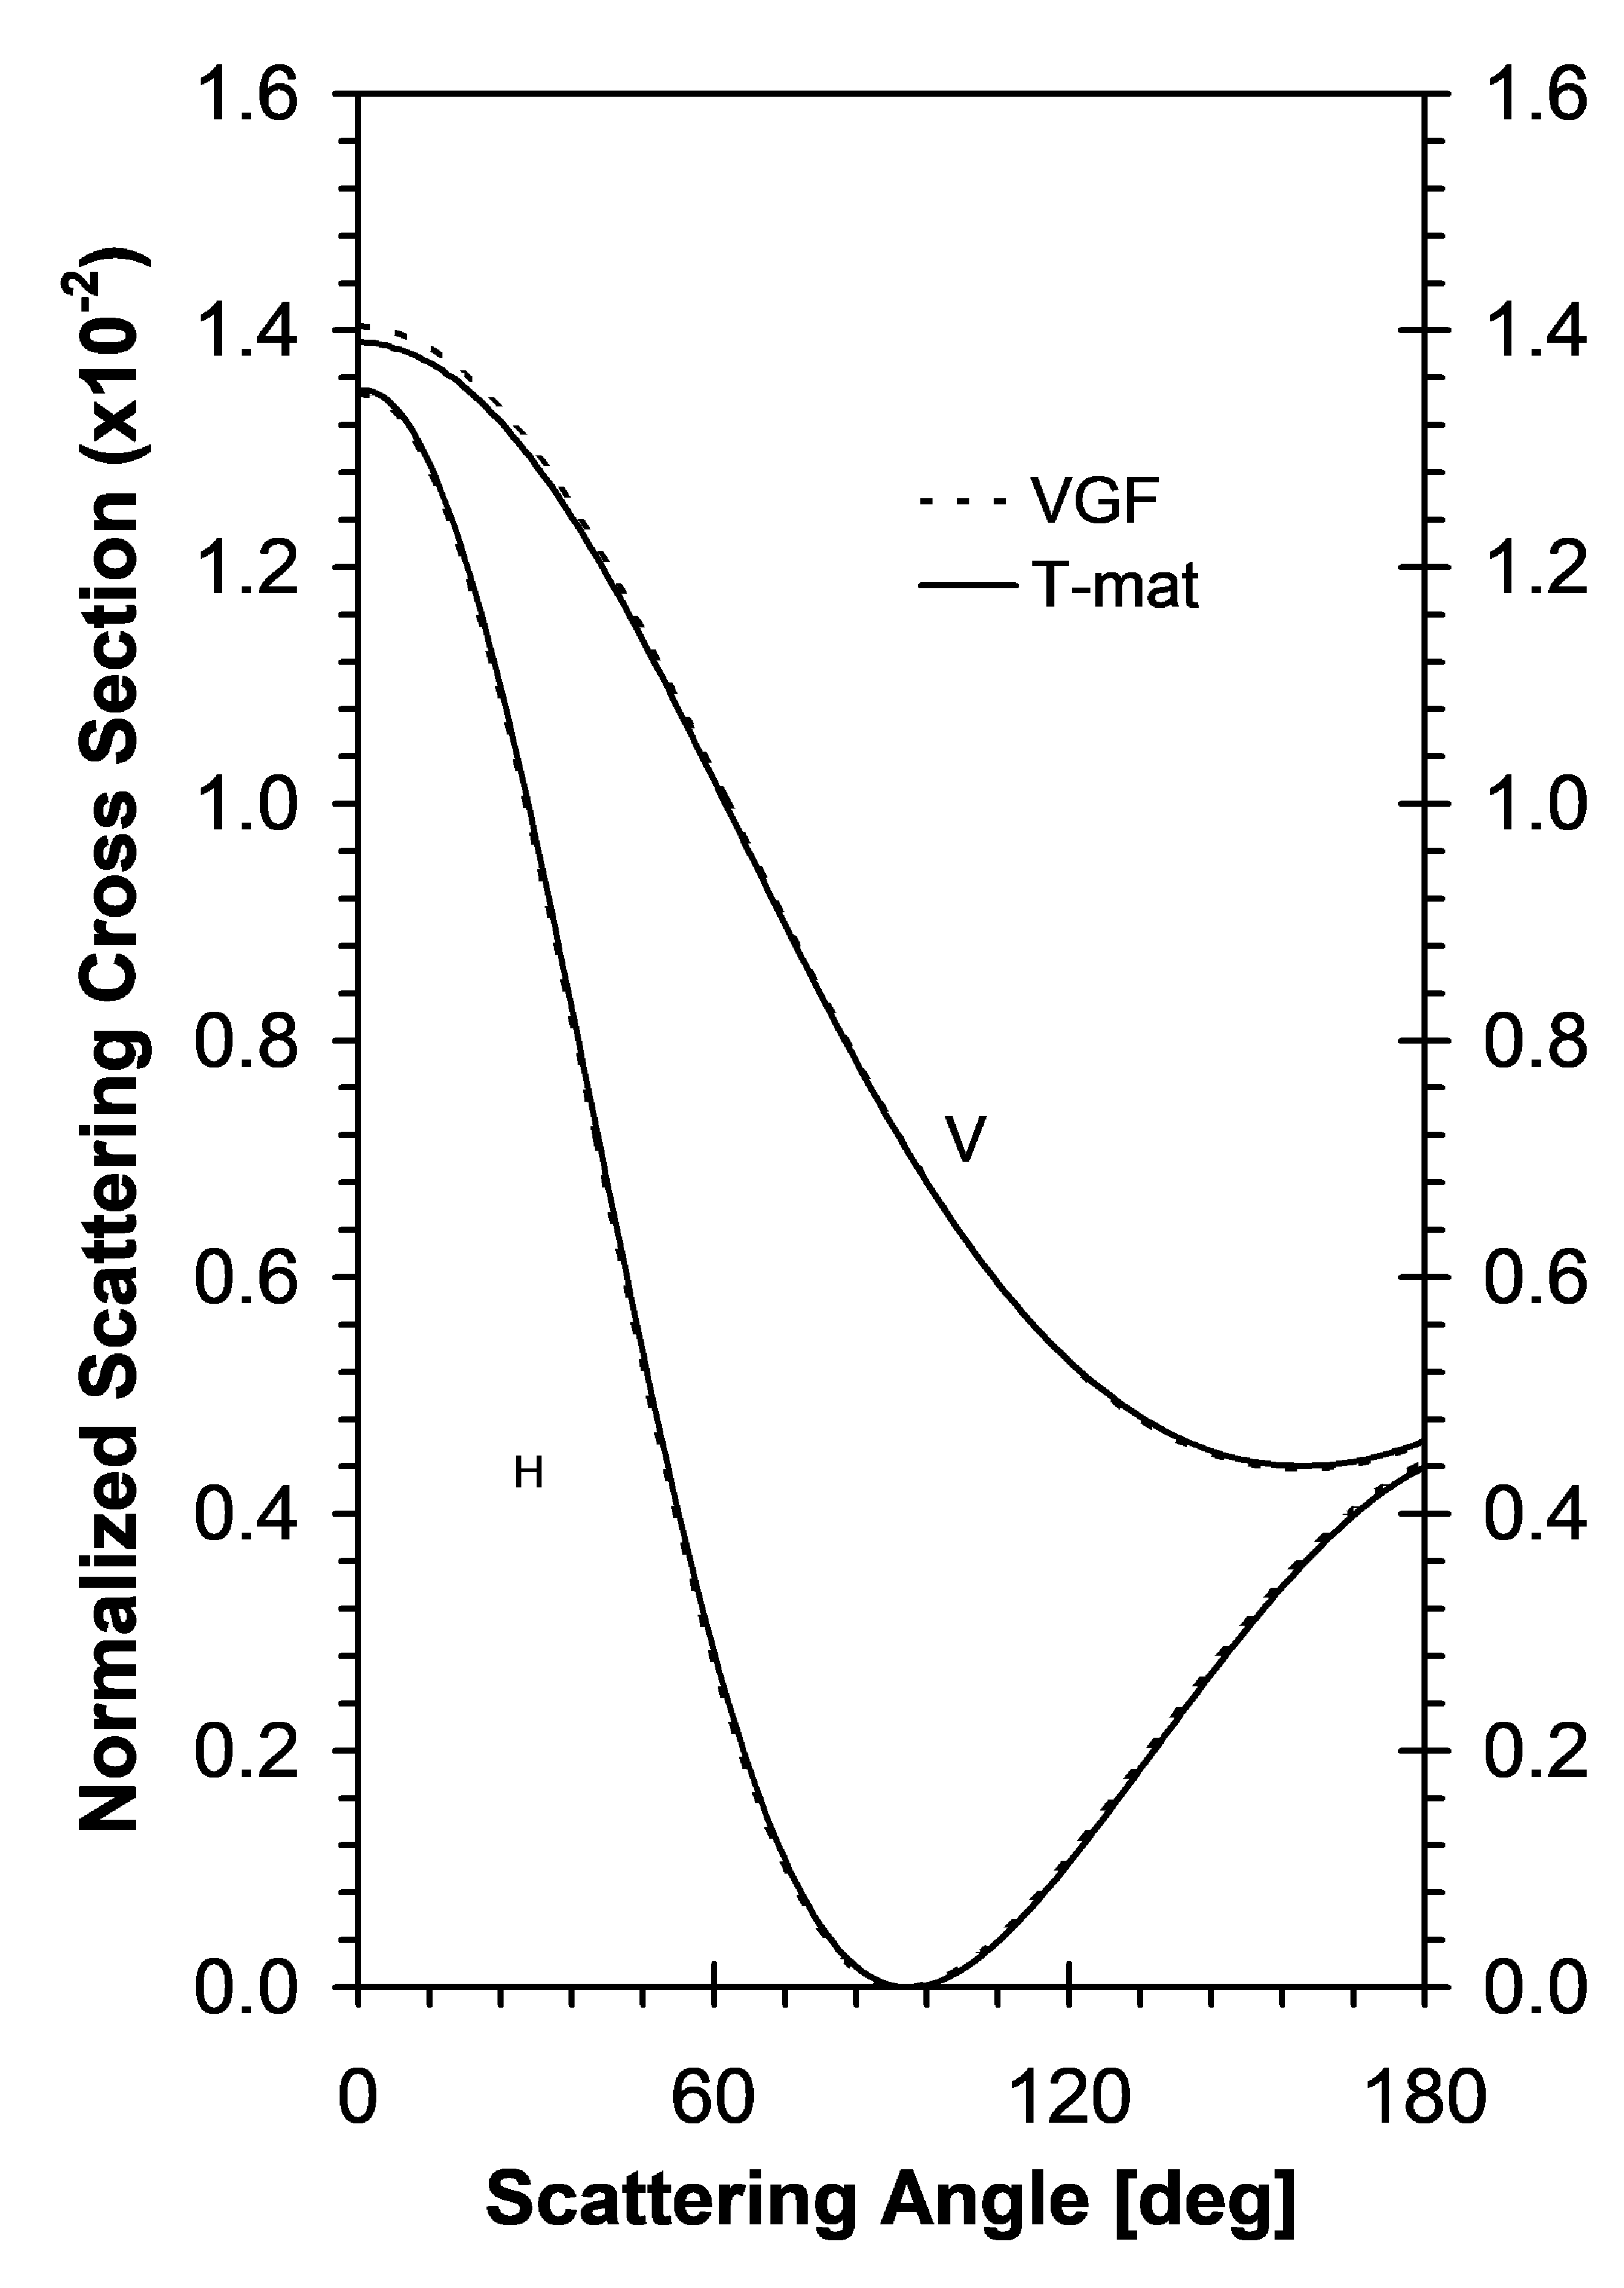
\includegraphics[width=0.8\linewidth, height=0.35\textheight]{test60b}
		\caption[short caption A]{A longer caption A}
	    \label{fig:bigsphere1}
	\end{minipage} \hfill
	\begin{minipage}{0.45\textwidth}
		\centering
		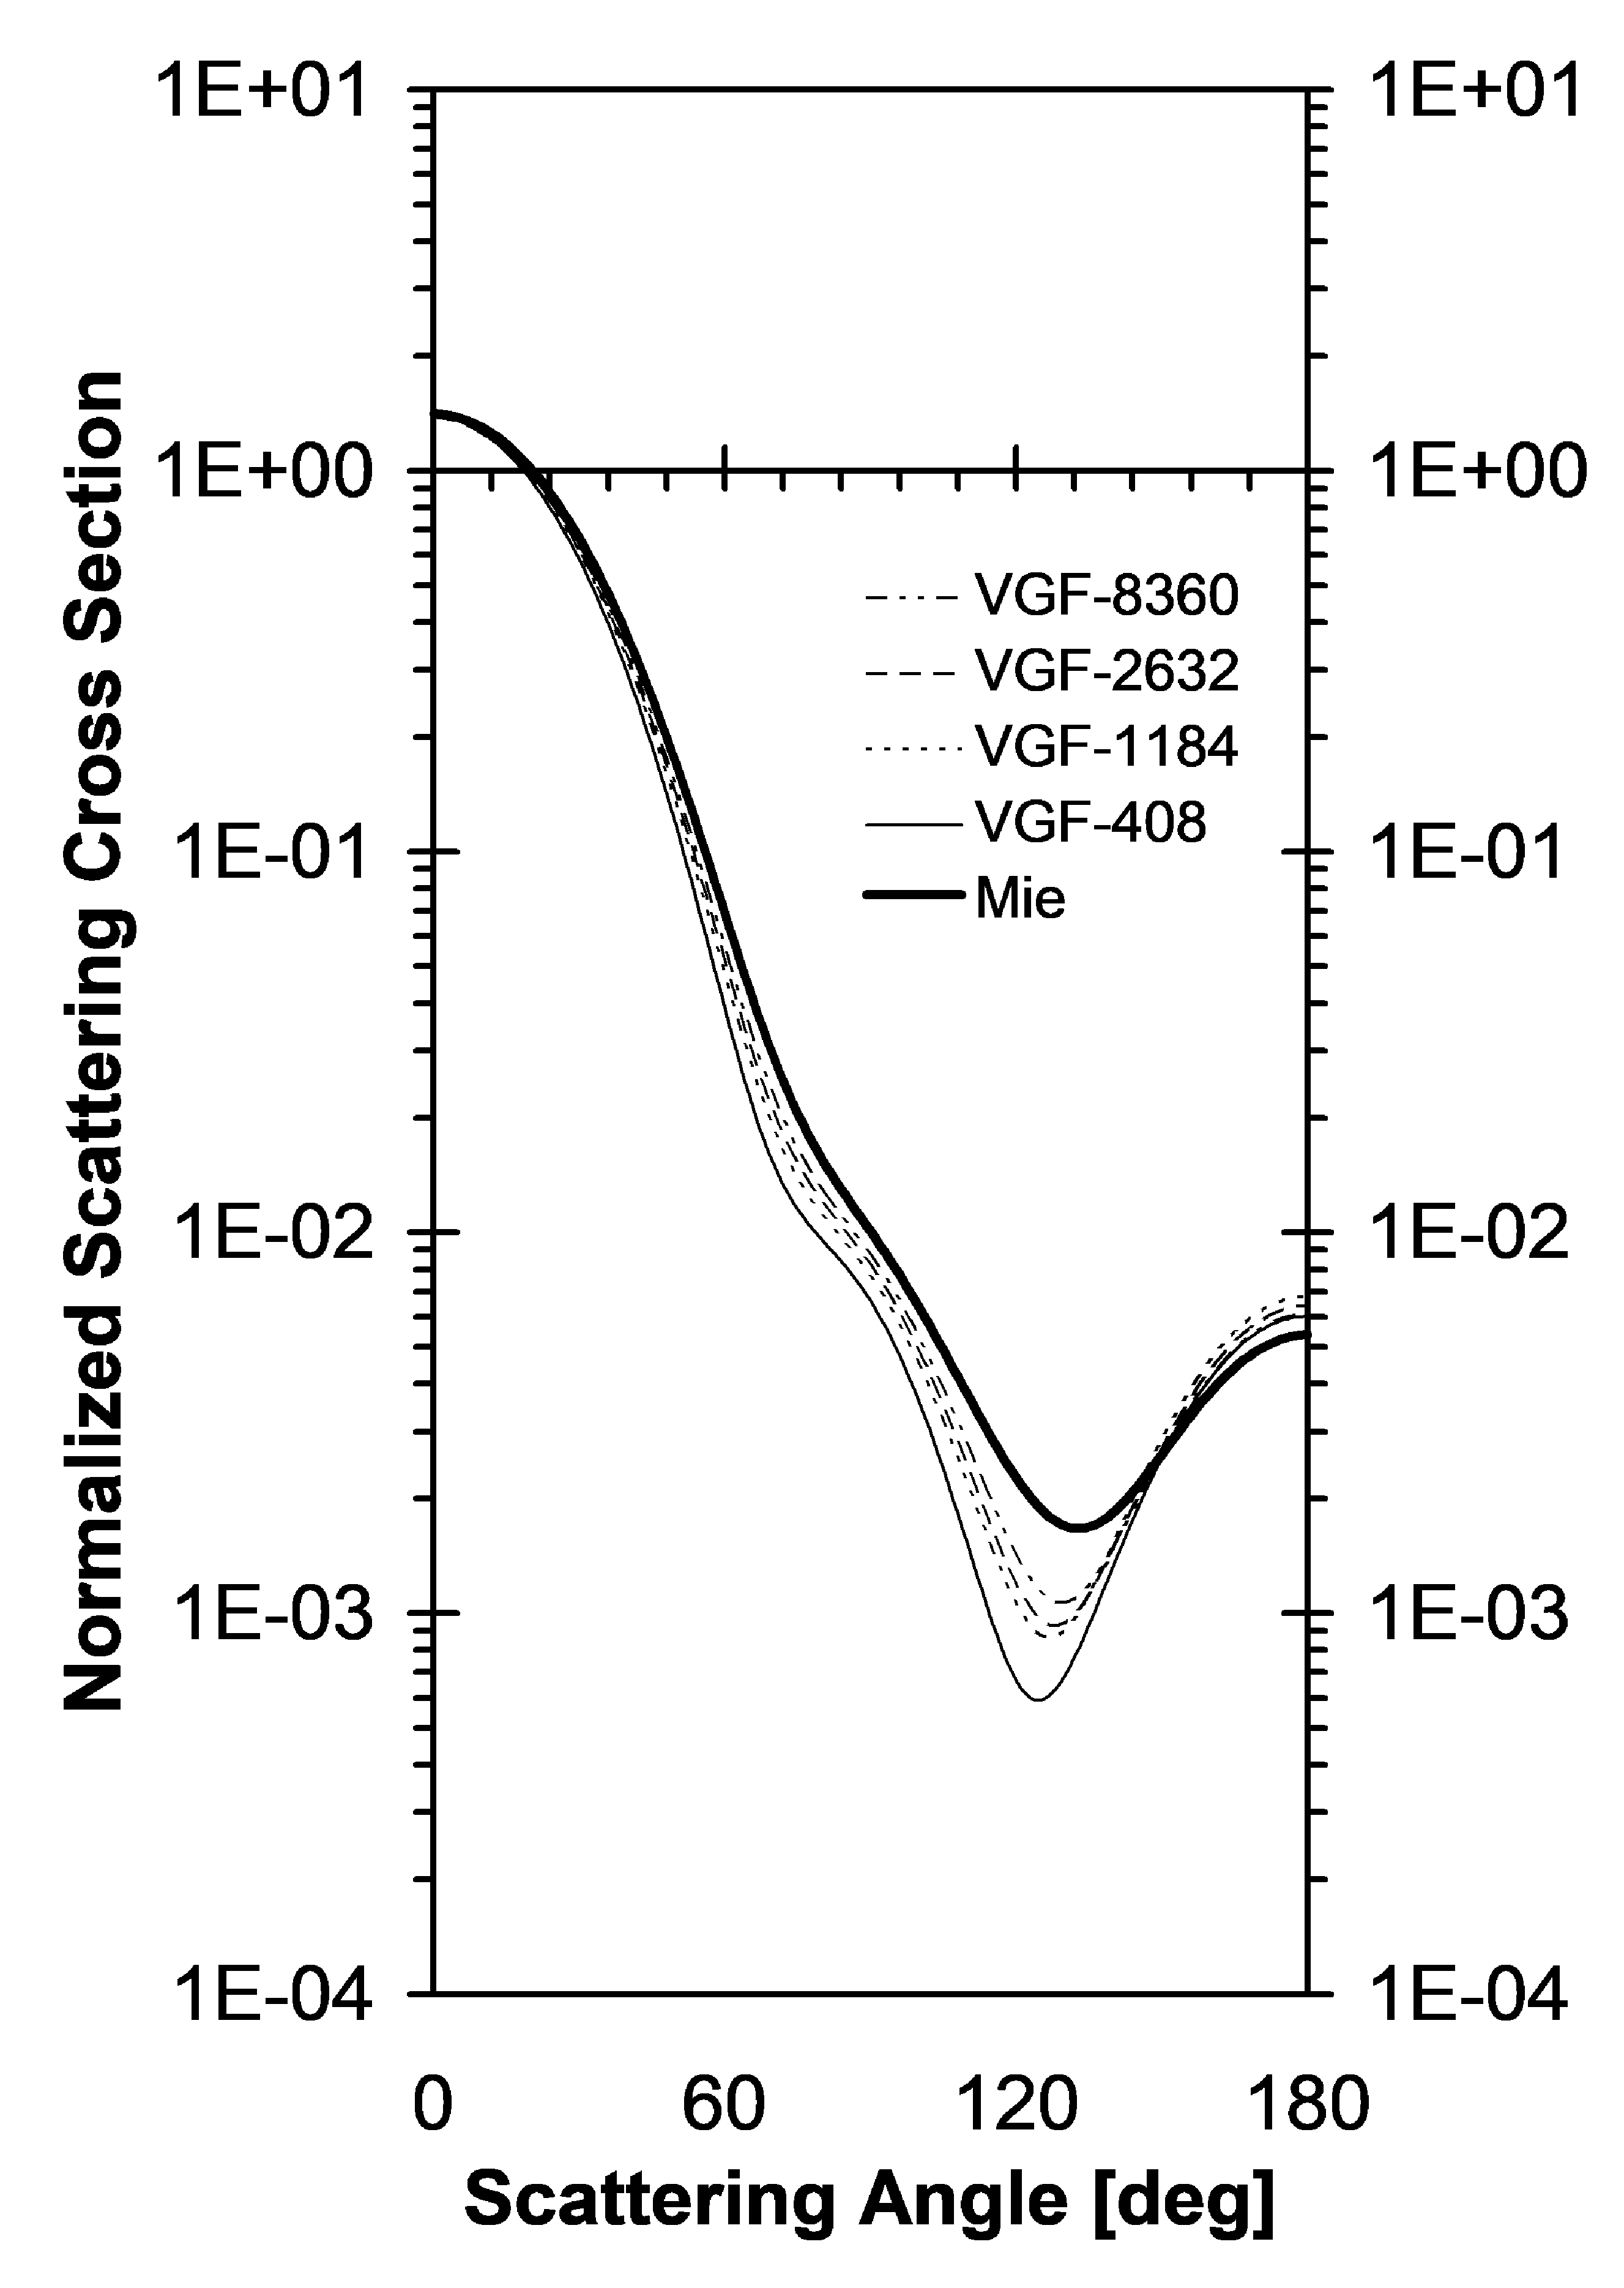
\includegraphics[width=0.9\linewidth, height=0.35\textheight]{test70}
		\caption{Caption b goes here}
		\label{fig:bigsphere2}
	\end{minipage}
\end{figure}
You might want to have different figures all as part of a larger figure. I recommend making the graphics as all one piece.  For example see figure \ref{fig:bigsphere1} and \ref{fig:bigsphere2}.
\section{defining new math operators}
This can be done with the following commands
\begin {verbatim}
   \DeclareMathOperator {\myOp}{myOp}
   \myOp(x)
\end{verbatim}
The first line needs to be in the preamble of your document. The second is put into math where you want the new operator to apperar. Then when you use the new operator it looks like this
$$\myOp(x)$$
Let's try this with erfc for the error function. Then we want to add 
\begin {verbatim}
\DeclareMathOperator {\erfc}{erfc}
\end{verbatim}
to the preamble and 
\begin {verbatim}
\erfc(x)
\end{verbatim} 
to the text where we want it.  It should look like this
$$\erfc(x)$$
or in the text $\erfc(x)$.
You might also want to put normal text in an equation. Like 
$$ \frac{x^2+distance^2}{r^2}$$
Note that the word ``distance'' doesn't look right. Using the 
\begin {verbatim}
   \textrm{normal text}
\end{verbatim}
command fixes this.
$$ \frac{x^2+\textrm{distance}^2 }{r^2}$$.
\section{Tables}
There is a lot to \LaTeX tables. I have more to write on this. But centering can be a difficulty.  Here are examples of doing that.

Example 1
Use the array package and define a new column type with horizontal or vertical centering (or both).  

\begin{verbatim}
	\newcolumntype{M}[1]{>{\centering\arraybackslash}m{#1}}
\end{verbatim} line above. Then in the column definitions in your table replace  the ``p'' with an ``M.'' 
\begin{table}[h]
	\centering
	\begin{tabular}[c]{|M{2.5cm}|M{1.5cm}|M{1.5cm}|M{1.5cm}|M{1.5cm}|M{1.5cm}|M{1.5cm}|} \hline
		Samples & \multicolumn{2}{|c|}{Data Item 1} & \multicolumn{2}{|c|}{Data Item 2} & \multicolumn{2}{|c|}{Data Item 3}\\ \hline
		Lifetime ($\tau$)     & 1     & 2     & 1     & 2     & 1     & 2     \\ \hline
		Average Lifetime (ps) & 116.5 & 464.2 & 114.7 & 404.7 & 115.3 & 414.7 \\ \hline
		Intensity (\%)        & 69    & 31    & 64.5  & 35.5  & 66.2  & 33.8  \\ \hline
	\end{tabular}
	\caption{This is the table caption}
	\label{OpenResults}
\end{table}

Example 2:
I use this one a lot.  Just put \textbackslash hfil  in each cell you want centered.

\begin{table}[h]
	\centering
	\begin{tabular}[c]{|p{2.5cm}|p{1.5cm}|p{1.5cm}|p{1.5cm}|p{1.5cm}|p{1.5cm}|p{1.5cm}|} \hline
			Samples & \multicolumn{2}{|c|}{Data Item 1} & \multicolumn{2}{|c|}{Data Item 2} & \multicolumn{2}{|c|}{Data Item 3}\\ \hline
		Lifetime ($\tau$)     & \hfil 1     & \hfil 2     & \hfil 1     & \hfil 2     & \hfil 1     & \hfil 2 \\  \hline
		Average Lifetime (ps) & \hfil 116.5 & \hfil 464.2 & \hfil 114.7 & \hfil 404.7 & \hfil 115.3 & \hfil 414.7 \\ \hline
		Intensity (\%)        & \hfil 69    & \hfil 31    & \hfil 64.5  & \hfil 35.5  & \hfil 66.2  & \hfil 33.8 \\ \hline
	\end{tabular}
	\caption{This is the table caption}
	\label{OpenResults}
\end{table}

Example 3:
The last example was a trick.  Maybe a ``better'' way to go is to put \textbackslash centering in the cells you want centered.

\begin{table}[h]
	\centering
	\begin{tabular}[c]{|p{2.5cm}|p{1.5cm}|p{1.5cm}|p{1.5cm}|p{1.5cm}|p{1.5cm}|p{1.5cm}|} \hline
		Samples & \multicolumn{2}{|c|}{Data Item 1} & \multicolumn{2}{|c|}{Data Item 2} & \multicolumn{2}{|c|}{Data Item 3}\\ \hline
		Lifetime ($\tau$)      & 1     & 2     & 1     & 2     & 1     & 2     \\  \hline
		Average Lifetime (ps)  & 116.5 & 464.2 & 114.7 & 404.7 & 115.3 & 414.7 \\  \hline
		Intensity (\%)         & 69    & 31    & 64.5  & 35.5  & 66.2  & 33.8  \\  \hline
	\end{tabular}
	\caption{This is the table caption}
	\label{OpenResults}
\end{table}


